\documentclass{beamer}
\usepackage{tikz}
\usepackage[utf8]{inputenc}
\usepackage{subcaption}
\graphicspath{{./}{images/}}
\usetheme{default}
\title{Programmation CUDA.}
\author{S. Puechmorel}
\date{2023}

\pgfdeclareimage[interpolate=true, height=0.155\paperwidth,width=\paperwidth]{bloc_enac}{images/Bloc_marque_RF_ENAC_V2.png}
\pgfdeclareimage[interpolate=true, height=40pt]{bloc2_enac}{images/Bloc_marque_RF_ENAC_V1.png}
\setbeamertemplate{background}{
  \begin{tikzpicture}
    \ifnum\thepage=1%
  \useasboundingbox (0,0) rectangle (\the\paperwidth,\the\paperheight); 
    \pgftext[at=\pgfpoint{0}{\paperheight-0.155\paperwidth},left,base]{\pgfuseimage{bloc_enac}};
    \else
\useasboundingbox (0,0) rectangle (\the\paperwidth,\the\paperheight); 
    \pgftext[at=\pgfpoint{0}{\paperheight-40pt},left,base]{\pgfuseimage{bloc2_enac}};
    \fi

  \end{tikzpicture}
}

\setbeamertemplate{frametitle}{
 \ifnum\thepage>1%
  \rightline{\insertframetitle}
 \fi   
}

\begin{document}
%1
\begin{frame}
    \titlepage

\end{frame}
%2
\begin{frame}
  \frametitle{Plan}
\tableofcontents
\end{frame}
\section{Historique.}
%3
\begin{frame}
    \frametitle{L'évolution des cartes graphiques.}
\begin{block}{Années 1980 : contrôleurs video.}
  Ces circuits permettaient d'afficher sur un tube cathodique 
  des informations stockées en mémoire. Ils fournissaient des fonctionnalités de base, essentiellement orientées
  autour de la gestion de la mémoire video et de la génération des signaux de synchronisation. 
  \begin{figure}[ht]
    \centering
    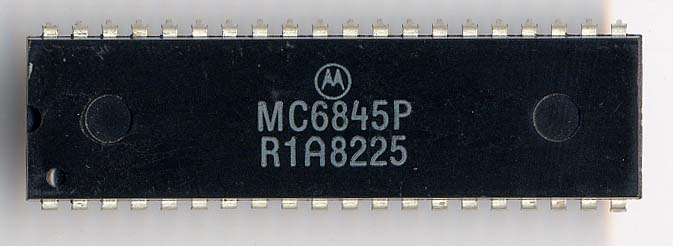
\includegraphics[scale=0.5]{Motorola_MC6845.jpg}
    \caption{Le contrôleur video MC6845. \footnote{\tiny \url{https://commons.wikimedia.org/w/index.php?curid=976920}}}
    \label{fig:MC6845}
  \end{figure}
\end{block}
\end{frame}
%4
\begin{frame}
  \frametitle{L'évolution des cartes graphiques.}
\begin{block}{Contrôleurs graphiques}
  Apparus vers la fin des années 1980, ils apportent des fonctionalités graphiques, telles le tracé de segment, et
   gérent une mémoire distincte de celle de l'unité centrale.
   \begin{figure}[htbp]
    \centering
    \hfill
   \begin{subfigure}{0.4\textwidth}
    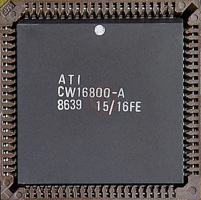
\includegraphics[scale=0.45]{ATI16800.jpg}
   \end{subfigure} 
   \hfill
   \begin{subfigure}{0.4\textwidth}
    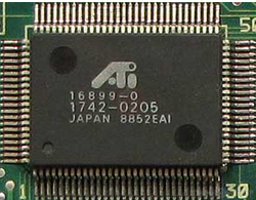
\includegraphics[scale=0.45]{ATI16899.jpg}
   \end{subfigure} 
   \hfill
    \caption{Contrôleurs graphiques.}
    \label{fig:graphic_controllers}
   \end{figure}
\end{block}
\end{frame}
\begin{frame}
  \frametitle{L' évolution des cartes graphiques.}
\begin{block}{Les processeurs graphiques.}
  
\end{block}
\end{frame}
\end{document}
